A study was carried out to choose the length of scintillating fibers that optimize the tritium detection efficiency. For this, the complete TRITIUM-Aveiro 0 prototype was simulated, in which the photon propagation was included.

First, the propagation of photons in scintillating fibers was studied. To do so,  the TRITIUM-Aveiro 0 prototype was simulated with a fibers length of $18~\cm$. The blue distribution of Figure \ref{fig:PhotonsFibersYesNoPhotosensors} shows the number of photons produced in the fiber per tritium event and the red distribution shows only the tritium events detected by the photosensors.

\begin{figure}[h]
\centering
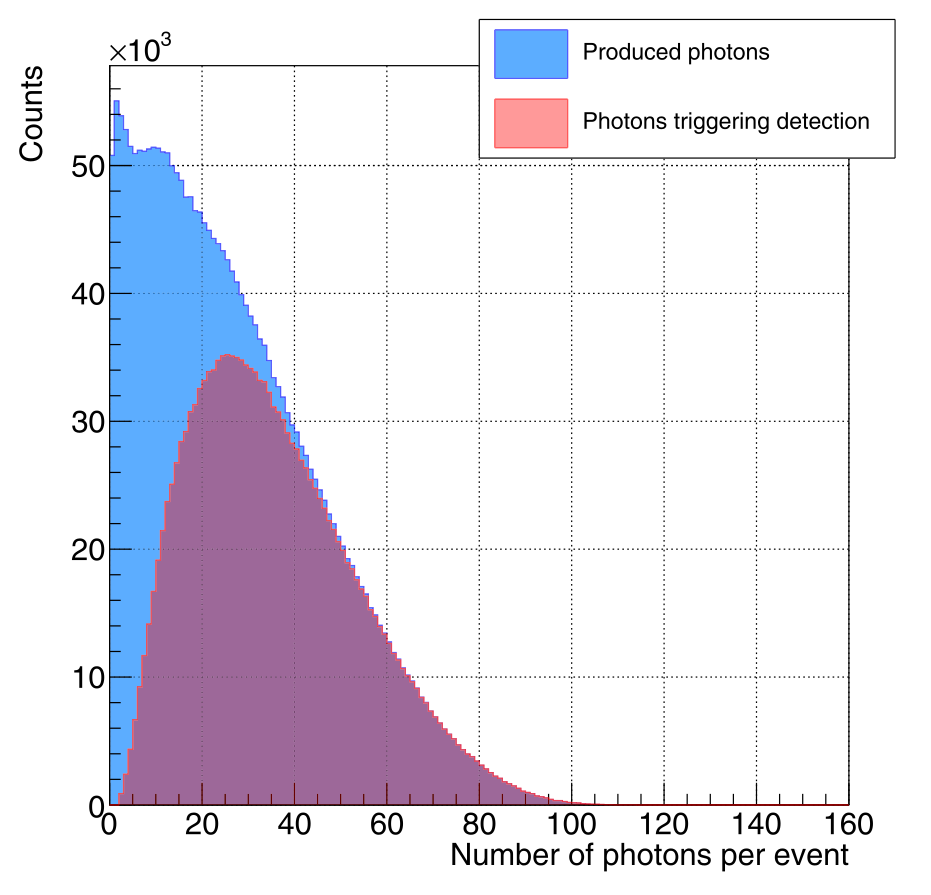
\includegraphics[scale=0.3]{Figures/8SimulationsResults/81TRITIUMDesign/813Length/CollectionPhotonsInFibers.png}
\caption{Number of photons produced in the fiber per tritium event for all tritium events that reach the fiber (blue histogram) and only for tritium events the photons of which are detected by photosensors (red histogram)\label{fig:PhotonsFibersYesNoPhotosensors}}
\end{figure}

It can be seen that tritium events with fewer photons produced in the fibers is not detected, producing a peak centred of around $25$ photons. This is mainly caused by the fiber collection efficiency. Tritium events that produce a high number of photons are practically always detected.

Regarding the fiber length study, two different lengths were compared, $1~\meter$ and $0.20~\meter$ and two different tritium source activity were used, $0.5~\kilo\becquerel/\liter$ and $2.5~\kilo\becquerel/\liter$. As detected tritium counts is proportional to the active area, 5 detectors were simulated, the results of which were summed, to normalize the study to the same active area.

The counts were integred  over $60~\min$ and taken over a week, the result of which is shown in Figure \ref{fig:CountsOver60minDifferentLength}.

\begin{figure}[h]
\centering
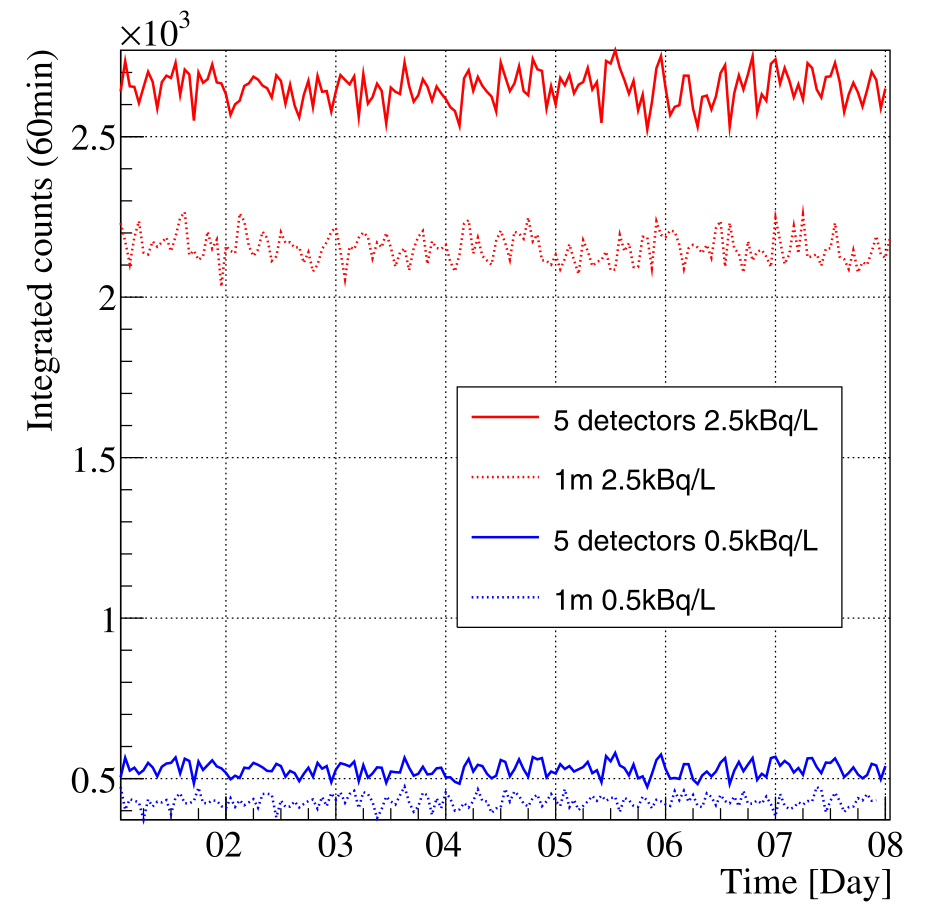
\includegraphics[scale=0.3]{Figures/8SimulationsResults/81TRITIUMDesign/813Length/2DifferentLength.png}
\caption{Counts integred over $60~\min$, normalized to the same active area and taken over a week for a fiber length of $1~\meter$, dashed lines, and $20~\cm$, solid lines and two different activities, $0.5~\kilo\becquerel/\liter$, blue lines, and $2.5~\kilo\becquerel/\liter$, red lines. \label{fig:CountsOver60minDifferentLength}}
\end{figure}

A larger signal is seen for shorter fiber lengths, producing a increasment in tritium detection efficiency of approximately $25\%$, principally produced by a lower absortion of scintillating fibers.

